% Allow relative paths in included subfiles that are compiled separately
% See https://tex.stackexchange.com/questions/153312/
\providecommand{\main}{..}
\documentclass[\main/thesis.tex]{subfiles}
\onlyinsubfile{\zexternaldocument*{\main/tex/introduction}}

\begin{document}

\chapter{Results}
\label{chap:nov_gen}
The proposed system for virtual drum generation proposed in Section~\ref{sec:thesis_statement} required the implementation of a virtual synthesizer and a virtual ear. The implementation and characteristics of these components were discussed in Chapters~\ref{chap:virt_synth} and~\ref{sec:ear} respectively. In this chapter, we discuss how the components are used to create generative systems of drum sounds. The labeled sounds created by the system are recorded on disk, allowing us to measure the success of this system by blinded, manual categorization of the outputs and calculating the level of agreement between categorical labels assigned by us and the labels assigned by the various ear models. 

\newcommand{\decfirst}{\textit{Decision.1}}
\newcommand{\decsecond}{\textit{Decision.2}}
\section{Putting The System Together}
 The virtual synthesizer generates a second of audio based on randomly generated programs, and the virtual ear can analyze the generated sounds and categorizes them as percussive or non-percussive. These two components work together to execute the plan laid out for the final, generative system of drum sounds, shown in Figure~\ref{fig:pipeline_outline}. A code example of how the system is put together is shown in Listing~\ref{lst:system_code}.

\begin{lstlisting}[float,floatplacement=H,caption={Example Program For The Generative System}\label{lst:system_code},captionpos=t]

import ear
import synthesizer
# randomly programming the synthesizer 1000 times 
while(i<1000):
    i+=1
    # stacksize is randomly selected from a list
    stack_size = random([1,2,4])
    # make synthesizer, randomly program it, generate sound
    sound = synthesizer.random_sound(stack = stack_size)
    # Check if ear determines sound to be percussive
    is_drum = ear.is_drum(sound)
    if is_drum:
        # give sound a drum category 
        drum_category = ear.drum_type(sound) 
        # save sound to hard_disk
        save_sound("path/to/drum_category/",sound) 
\end{lstlisting}

This loop runs in a single CPU process, therefore generation can scale-up easily. Here, sounds are rapidly generated and sent to the virtual ear, which then separates drums from non-drums. The sounds labeled as drums are further analyzed and assigned a drum type. Finally, the accepted sounds are saved to hard-disk for use in compositions. In this chapter, we cover the results of our blinded, manual hearing tests conducted on the sounds generated by these two systems.

\label{gens}
\label{surveys}
\section{How and Why Surveys are Conducted}
 
 The main function of the manual hearing tests is to measure the precision of the virtual ear when the model is performing open-set recognition, i.e, separating drums sounds from none-drum sounds. If a small subset of synthetic noise can stand in for percussive sounds, then the ideal synthetic ear will be able to separate the desired sounds from noise with high recall and precision (see Figure~\ref{fig:ven_data}). Low recall will cause a slow-down of the pipeline, as a larger number of random sounds need to be generated and evaluated. Low recall is also likely to increase the loss of novel sounds. Low precision will make manual clean-up of generated samples necessary and arduous. 

To assess the performance of each pipeline, we randomly create drum programs and generate the corresponding audio signal. This sound is then fed through the ear model to determine if the sound is percussive. If so, a category is assigned to the sound. This sound and the corresponding synthesizer program are saved to hard-disk. Here we assess the success rate of two different pipelines by manual inspection and categorization of a randomly selected subset of its results. We cross reference the manual categorizations with the categories assigned by the virtual ear and seek to answer the following two research questions for each system: 
\begin{itemize}
\item \textbf{RQ.1}: Do we agree that the sounds are percussive? 
\item \textbf{RQ.2}: Do we agree with the drum category assigned to the percussive sounds?
\end{itemize}
 \section{Survey of Two-Phased Ear Performance}
   

%  We put a generative system together using a TPE ear. When using CPU, each loop could take up to 200 ms, however, each loop can be run on a simple process and multiprocessing can easily speed up generation time. Here, approximately 300 loops were necessary to create a drum sound, however, slight variations in recall and precision can change this number significantly. 
 
 \subsection{Methodology and Dataset}
  To answer \textbf{RQ.1} and \textbf{RQ.2} for the TPE approach, we put a generative system together using the TPEs discussed in Section~\ref{TPE_models}, and ran the system until a large number of samples in each category were found and saved to disk. Next, we randomly picked around 50 samples in the following categories: \enquote{snare}, \enquote{kick}, \enquote{hat}, \enquote{clap} and \enquote{other} (combination of rims, 
shakers and unusual percussive sounds). This gave us a total of 257 samples. These samples were determined to be percussive and then categorized by 3 different drum vs drum models (FC, CNNLSTM, E+F). We ensured a balanced division between samples of stack size 1, 2 and 4 (each stack is responsible for a third of the samples under each category).
 \subsection{Survey Application and Results}
Amir Salimi and Abram Hindle categorized these samples without knowledge of each other's results, or drum categorizations assigned by the virtual ears. It's important to note that each responder had an additional category of \enquote{Bad} for samples that they deemed not percussive. The \enquote{Bad} category indicates that the sample should have not been accepted as percussive.


\begin{figure}[tbp]
    \begin{center}
    \textbf{Label Assignment Frequency For TPE Survey}
    \makebox[\textwidth]{
    \includegraphics[width=1.1\linewidth]{images/chapter_4/cat_2p_fixed.pdf}}
    \end{center}
    \caption{Frequency of assigned labels by persons versus the true number of labels (for TPEs)}
\label{fig:freq-survey-2p}
\end{figure}
We assess the reliability of agreement between persons and categorization models via the Fleiss' kappa coefficient \cite{fleiss1971measuring}. The value of 0 or less for this coefficient indicates no agreement beyond random chance, and the value of 1 indicates perfect agreement. Our kappa measurements shown in Table~\ref{kappa_table_TPE} lie within the 0.35-0.45 range, indicating mild to moderate agreement between persons and machines. We again measure this coefficient after dropping samples that were categorized as \enquote{Bad} by the authors, as samples that persons deem to be \enquote{Bad} should not have been categorized by the models at all. Dropping of samples that both authors deemed \enquote{Bad} causes an 8\% reduction of our data (21 samples) and a small increase in kappa score. Dropping samples deemed \enquote{Bad} by either reviewer resulted in a 30\% reduction of samples and relatively large increase in kappa scores. 
\begin{table}[tbp]
 \resizebox{\linewidth}{!}{\begin{tabular}{||c c c c c c c||} 
 \hline
 Drop Rule & Size & H+H & H+FC & H+CNN & H+E/F & 3 models \\ [0.5ex] 
 \hline
 No Drops & 257 &0.37 & 0.35 & 0.36 & 0.36 & 0.28\\ 
 \hline
 Assigned \enquote{Bad} By Both & 236 & 0.31 & 0.37 & 0.37 & 0.38 & 0.30 \\
 \hline
 Assigned \enquote{Bad} By Either & 180 & 0.47 & 0.50 & 0.48 & 0.48 &  0.34 \\
 \hline
 Assigned \enquote{Bad} or \enquote{Other} By Either & 154 & 0.47 & 0.59 & 0.54 & 0.50 &  0.35 \\
 \hline
\end{tabular}}
\caption{\label{kappa_table_TPE}Table of Fleiss' kappa coefficients to measure the degree of agreement between persons (HvH) and various TPEs: persons with FC model (H+FC), persons with CNNLSTM model, persons with all models (H+E/F), and between the 3 models. \enquote{Drop Rule} column indicates if any samples were dropped. We show the measurements after dropping samples if they are deemed bad by either or both responders. We also show measurements after dropping the \enquote{other} category along with samples deemed bad by either responder. }
\end{table}
\subsection{Takeaways Of The TPE Pipeline Survey}
Our main takeaways from the TPE survey are as follows:
\label{survey1_takeaway}
\begin{itemize}
    \item For \textbf{RQ.1}, the survey brings into question the reliability of our DVN models, as 30\% of the generated samples were deemed not percussive by at least 1 reviewer and 8\% by both reviewers. 
    \item For \textbf{RQ.2}, the task of categorizing synthetic drums appears difficult. Survey shows that even after removal of \enquote{Bad} samples, the scale of agreement between just 2 persons (H+H) as well as between 2 persons and any of the models (H+FC, H+CNN, H+E/F) is moderate at best; while the same models can achieve over 98 percent accuracy when tested on recorded drum samples. This may be a manifestation of the \enquote{open set recognition} problem. 
    \item While there is much room for improvement, our pipeline can generate and categorize drums and percussive sounds with a promising degree of success. 
\end{itemize}

 \section{Survey of Mixed Ear Model Performance}
  \subsection{Methodology and Dataset}
  To answer \textbf{RQ.1} and \textbf{RQ.2} for the MEM approach, we kept the other components of the pipeline the same, while using the MEM as the virtual ear. With TPEs, the~\enquote{other} category is assigned when the sound is determined to be percussive in the first phase, but the second phase determines that the sound does not belong to any of the drum categories it is familiar with. MEMs either assign the sound to a drum category or determine that it is not a drum, therefore the MEM survey differs from the TPE survey in that the pipeline only creates the four drum categories, yet the \enquote{other} category can still be assigned by survey responders. This means that two out of six possible categories are only available to responders, which can cause an inherent bias towards worse agreement scores compared to the last survey. 
 \subsection{Survey Application and Results}
 \begin{table}[tbp]
 \resizebox{\linewidth}{!}{\begin{tabular}{||c c c c||} 
 \hline
 Drop Rule & Size & HvH & H+MEM \\
 \hline
 No Drop & 300 & 0.336 & 0.250\\ 
 \hline
 Assigned Bad By Both & 249 & 0.200 & 0.260 \\
 \hline
 Assigned Bad By Either & 151 & 0.460 &  0.473 \\
 \hline
Assigned \enquote{Bad} or \enquote{Other} By Either  & 120 & 0.620   &  0.587 \\
 \hline
\end{tabular}}
\caption{\label{kappa_table_MEM}Table of Fleiss' kappa coefficient to measure the degree of agreement between persons (HvH) and persons and MEM. We measure the agreeability scores after dropping bad samples if both or either persons assigned the sample as such. We also measure agreeability when all samples deemed \enquote{Bad} or \enquote{other} by either person are removed.}
\end{table}

\begin{figure}[tpb]
    \begin{center}
    \textbf{Category Assignment Frequency For MEM Survey}
    \makebox[\textwidth]{
    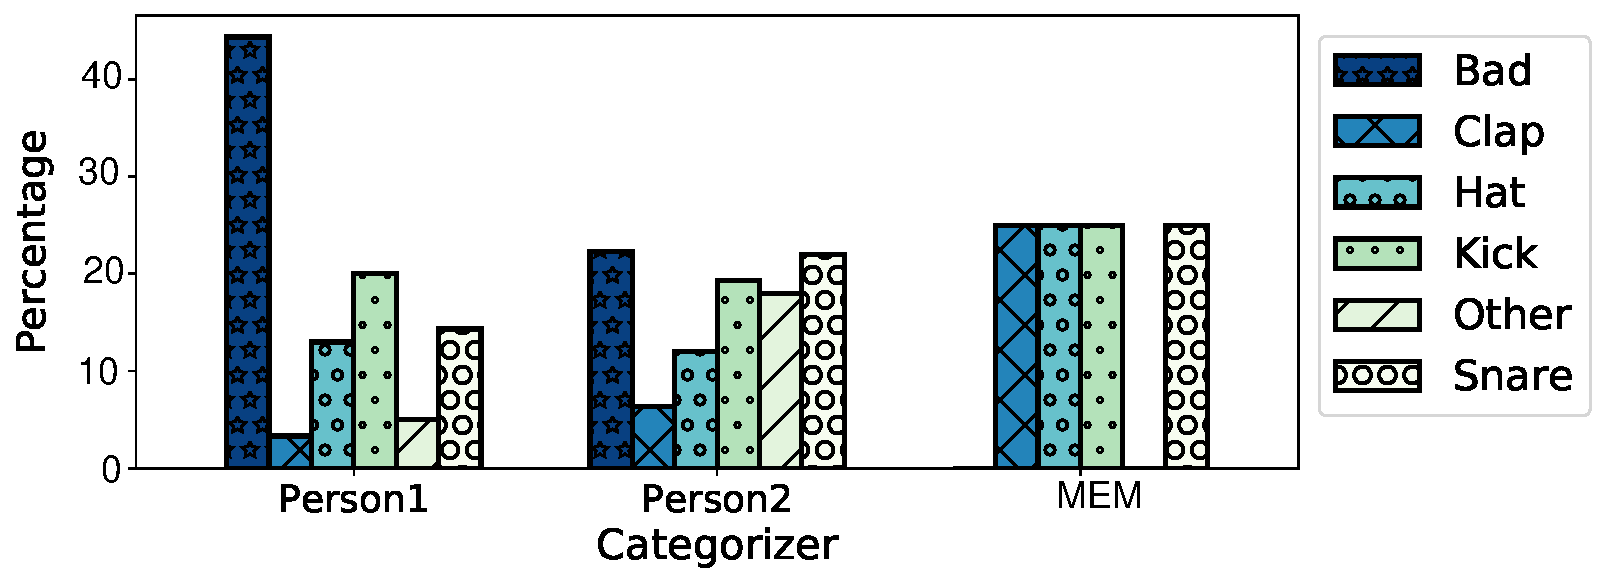
\includegraphics[width=1.1\linewidth]{images/chapter_4/cat_mme_fixed.pdf}}
    \end{center}
    \caption{Frequency of assigned labels by persons versus the true number of labels (for MEMs)}
\label{fig:freq-survey-2p}
\end{figure} 

 As shown in Table~\ref{kappa_table_MEM}, before dropping the~\enquote{bad} outputs, there is mild to moderate agreeability. By dropping~\enquote{bad} samples (therefore accounting for failures in~\decfirst), a dramatic increase in agreeability score is seen in the results.  This highlights a the MEM's weakness in the separation of drums from non-drums. 

% Tables~\ref{kappa_table_TPE} and~\ref{kappa_table_MEM} depict the agreeability scores under different drop rules. The scores for the MEM pipeline are often lower, but we reiterate that this can be caused by having two out of six (rather than one out of six in the TPE pipeline) categories which are exclusive to survey responders. Supporting this hypothesis is the notable improvement in agreeability observed after dropping all \enquote{Bad} and \enquote{other} samples. Here, both persons agree with each other and the MEM at a stronger rate than in the TPE pipeline, despite having similar number of samples (120 for MEM and 154 for TPE) and equal number of categories to choose from. These values are observed in the last rows of Tables~\ref{kappa_table_TPE} and~\ref{kappa_table_MEM}. 

\subsection{Takeaways Of The MEM Pipeline Survey}
\label{survey2_takeaway}
Our main takeaways from the MEM survey are as follows:
\begin{itemize}
\item For \textbf{RQ.1}, 50\% of sounds were deemed~\enquote{bad} by at least one survey taker, and 17\% by both.
\item For \textbf{RQ.2}, the improvement in kappa scores after reduction of~\enquote{bad} outputs show that similar to TPEs, mistakes in separation of drums in non-drums is a major point of failure. 
\item Overall, these results show success in usage of spectrogram autoencoders as feature extractors for sounds, however we suspect that open set recognition is a major weakness. 
\end{itemize}

\section{Survey Conclusion}
\label{survey-conc}
The results highlighted here are encouraging, as 50\% or more of the outputs from either pipeline is deemed percussive by both survey takers, and moderate to high agreement between human and virtual listeners is observed for both \decfirst~and~\decsecond. A comparison of the survey results helps identify common weaknesses and avenues for improvement in the future. By using agreeability scores as the performance measure, we compare the two models with regards to separation of drums from non-drums and categorization of drum types:
\begin{itemize}
\item \textbf{Decision 1:} The sounds generated were deemed percussive by both subjects in 70\% of the cases with the TPE system, and 50\% with the MEM. This discrepancy is highlighted  in the agreement scores as well; The agreement scores in Tables~\ref{kappa_table_TPE} and~\ref{kappa_table_MEM} show the scores before and after failures in~\decfirst~were removed according to various rules. Here, we see a sharper increase in the agreeability scores for the MEM as more failures in drum vs non-drum separation are removed. This further highlights that~\decfirst~is a more pronounced weakness for the MEM.
\item \textbf{Decision 2:} When all \enquote{bad} and \enquote{other} sounds are removed, the models can be fairly compared for their performance in~\decsecond. Here, the MEM matches the performance of FC, the best drum categorizing TPE. This suggests that drum classification using spectrogram embeddings can match or exceed the performance of models which learned from the entire spectrogram. This is interesting as the autoencoder model used for feature extraction was trained for encoding spectrograms into a small, 8-dimensional feature space and recreating the original using said features, not feature extraction for drum classification. Yet this feature space proves useful in drum-classification, although not in drum vs non-drum classification.  
\end{itemize}

Overall, the OSR problem (as described in Section~\ref{sec:ear_caveats}) is a major weakness in this project, particularly in the MEM approach. When removing all failures in~\decfirst, the agreeability scores of the MEM and the best TPE are comparable and within a satisfactory "moderate to strong agreement" kappa range for~\decsecond. However, despite these failures, the approach taken in this work has enabled the generation of virtually synthesized drum sounds in an unsupervised manner, achieving the original goal of the project outlined in the thesis statement in Section~\ref{sec:thesis_statement}. 


% \begin{lstlisting}[language=Python]
% import TPE_System
% drum_kit = {}

% TPE_System.generate_drums(drum_kit)

% \end{lstlisting}

\end{document}